\section{Use cases}

\begin{figure}
  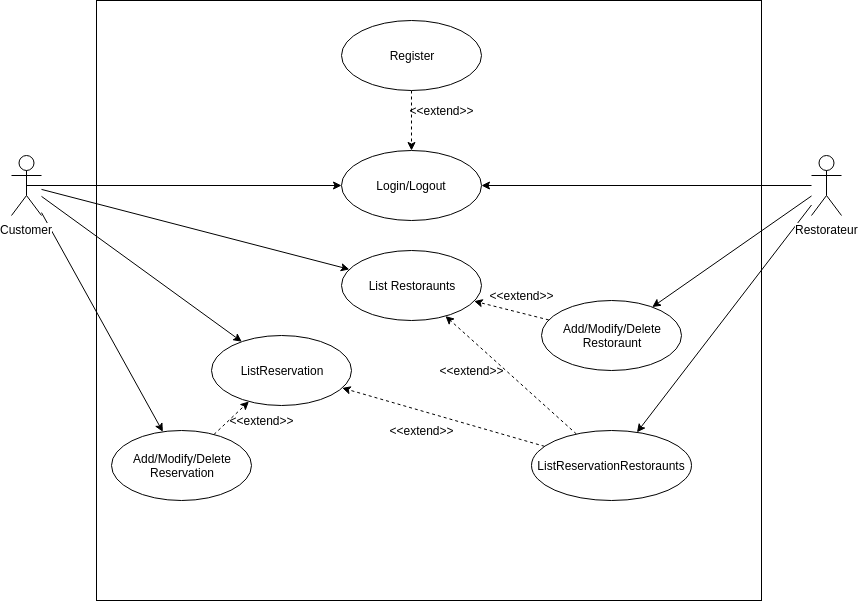
\includegraphics[width=\linewidth]{USE_CASE.png}
  \caption{Use cases diagram.}
  \label{figureUSE_CASE}
\end{figure}

	\begin{enumerate}
		\item Registration: The first time a user uses the application  he/she will be asked to register himself/herself, providing an username and a password, and specifying which type of user he/she is (customer or restaurant owner).
		\item Login: A User (customer or restaurant owner), will provide his credentials, the application will check if he/she is in the system and then will grant or deny the access, depending on the result of the check.
		\item Browse Restaurant: The list of all available restaurant, with description, genre, price, and number of seats available. the list is provided to  customers from which they can choose the restaurant to book.
		\item Browse Reservation: The list of all the reservations made. For a customer, it is the list of their reservations made for different restaurants. For the restaurant owner, this is the list of reservations made by customers in their restaurant.
		\item Add Restaurant: \textbf{?????????????????????????????}
		\item Modify Restaurant: a restaurant owner is able to modify a restaurant.
		\item Add Reservation: customer can make a reservation at one of the available restaurants.
		\item Delete Reservation: customer can delete a reservation made in the past.
	\end{enumerate}

\pagebreak